In this chapter, the simulations carried out are documented.

The \dq Xpedition AMS\dq\ tool from Siemens is used for the simulation. As the name suggests, this tool supports
\acrfull{ams} analysis. \cite{siemens2025xpeditionams}

\subsection{Laser Driver}

Figure~\ref{fig:simulation_laser_driver_schematic} shows the schematic for the laser driver simulation.
This corresponds to the circuit from chapter~\ref{sec:schematic_laser_driver}.

\begin{figure}[H]
    \centering
    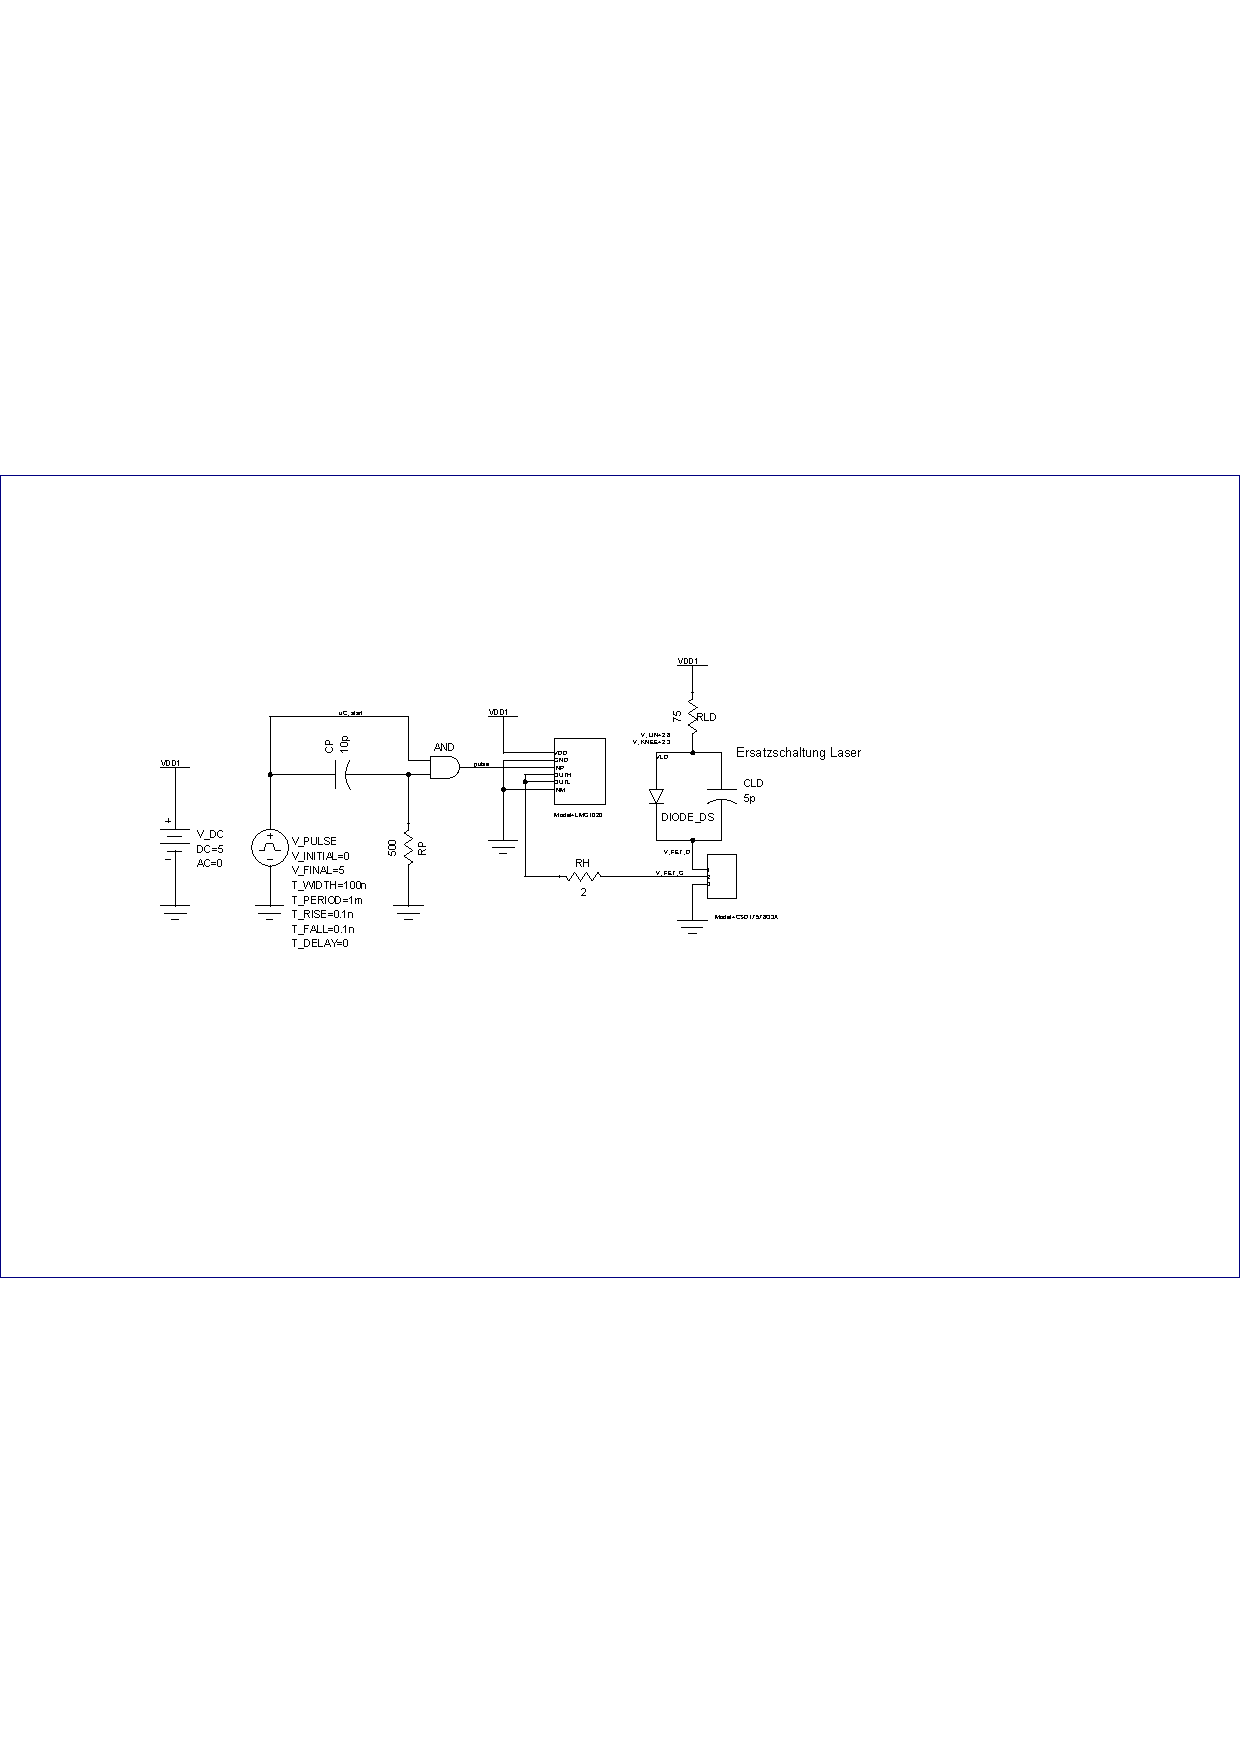
\includegraphics[trim=70 380 180 310, clip, width=0.9\textwidth]{../attachments/simulation_laser_driver_schematic.pdf}
    \caption{Simulation Laser Driver - Schematic}\label{fig:simulation_laser_driver_schematic}
\end{figure}

The SPICE model of the gate driver LMG1025-Q1 is the same as for LMG1020 and was downloaded from the TI website
\cite{ti2024lmg1025q1}.

The SPICE model of the NexFET CSD17578Q3A was also downloaded from the TI website
\cite{ti2024csd17578q3a}.

No SPICE model could be found for the laser diode RLD65NZX1, so an equivalent circuit consisting of a diode
and a parallel parasitic capacitance was inserted.

The result of the simulation is shown in Figure~\ref{fig:simulation_laser_driver_plot}.

\begin{figure}[H]
    \centering
    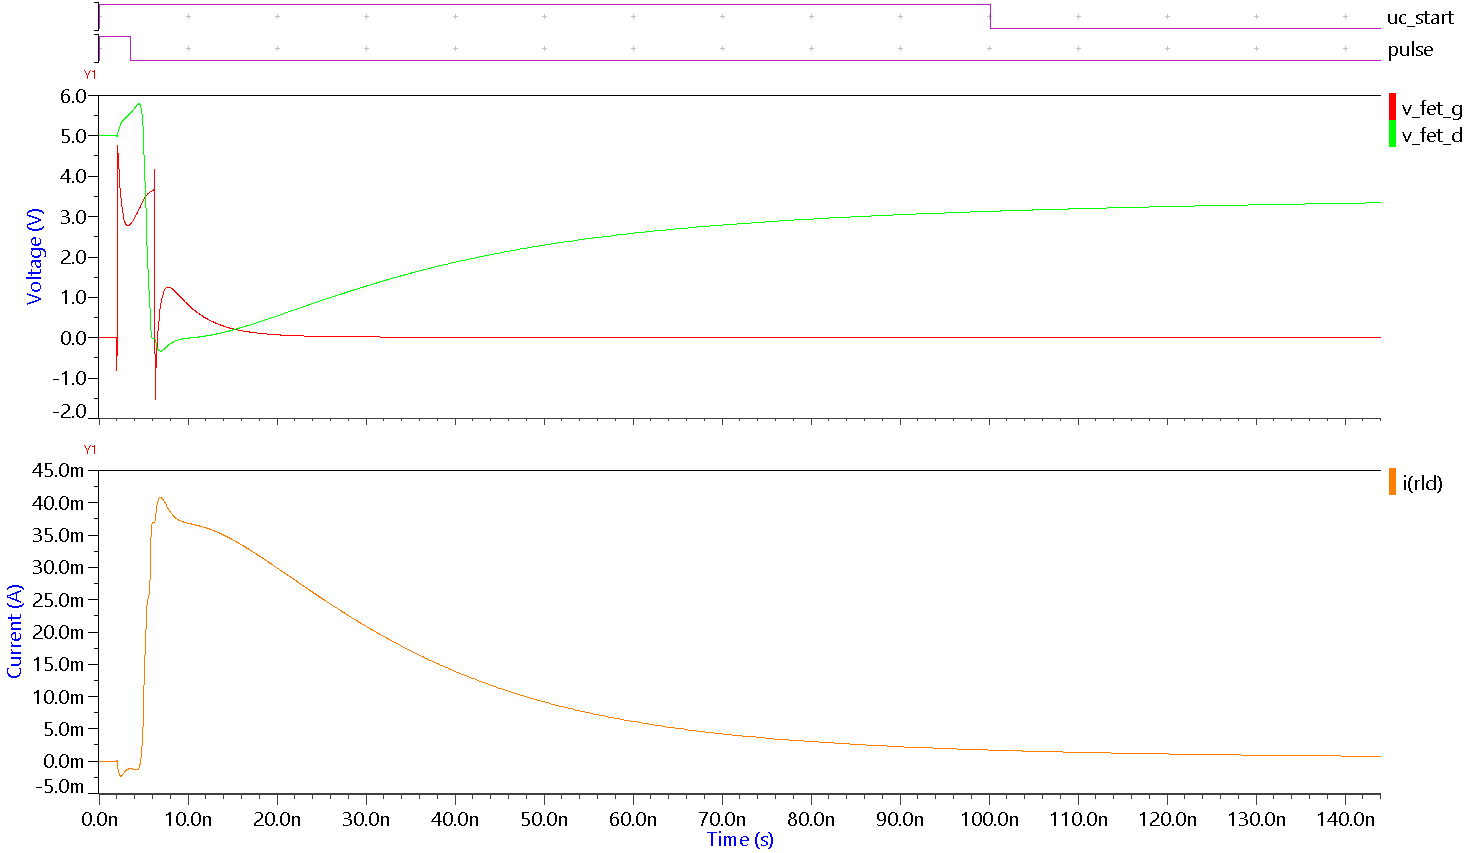
\includegraphics[width=\textwidth]{../graphics/simulation_laser_driver_plot.png}
    \caption{Simulation Laser-Driver - Plot}\label{fig:simulation_laser_driver_plot}
\end{figure}

It can be seen that the laser can switch on very quickly (2 \dots 3~ns). Switching off takes a little longer
(about 100~ns). Since the \acrshort{tof} is measured up to the first edge, a longer switch-off time is
not a problem for this application.

\subsection{Transimpedance amplifier}

Figure~\ref{fig:simulation_tia_schematic} shows the schematic for the simulation of the transimpedance amplifier. This
corresponds to the circuit from chapter~\ref{sec:schematic_photo_receiver}, without the comparator.

\begin{figure}[H]
    \centering
    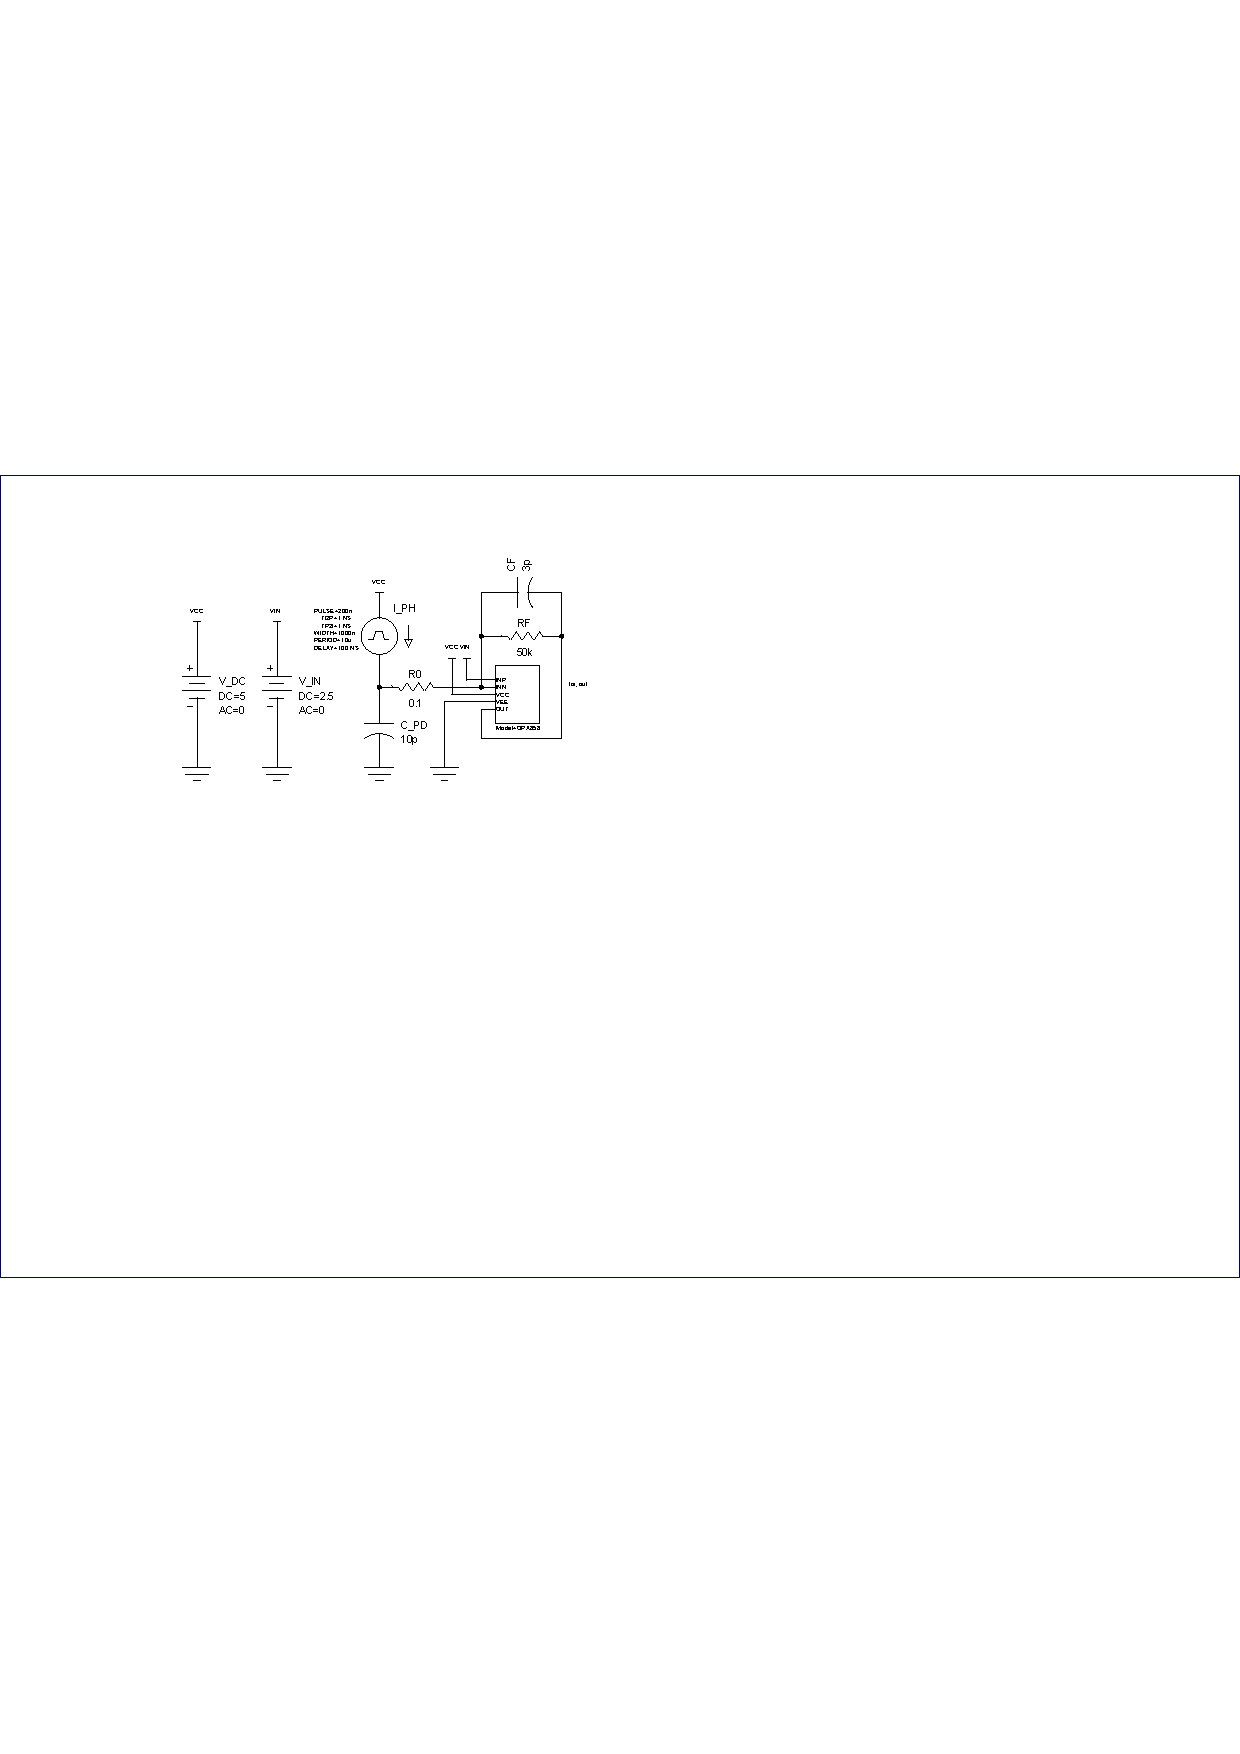
\includegraphics[trim=80 465 310 265, clip, width=0.7\textwidth]{../attachments/simulation_tia_schematic.pdf}
    \caption{Simulation \acrshort{tia} - Schema}\label{fig:simulation_tia_schematic}
\end{figure}

The SPICE model of the operational amplifier OPA858 was downloaded from the TI website \cite{ti2024opa858}.

No SPICE model could be found for the photo diode NJL6401R, so an equivalent circuit consisting of
a current pulse source and a parallel parasitic capacitance was inserted.

The result of the simulation is shown in Figure~\ref{fig:simulation_tia_plot}.

\begin{figure}[H]
    \centering
    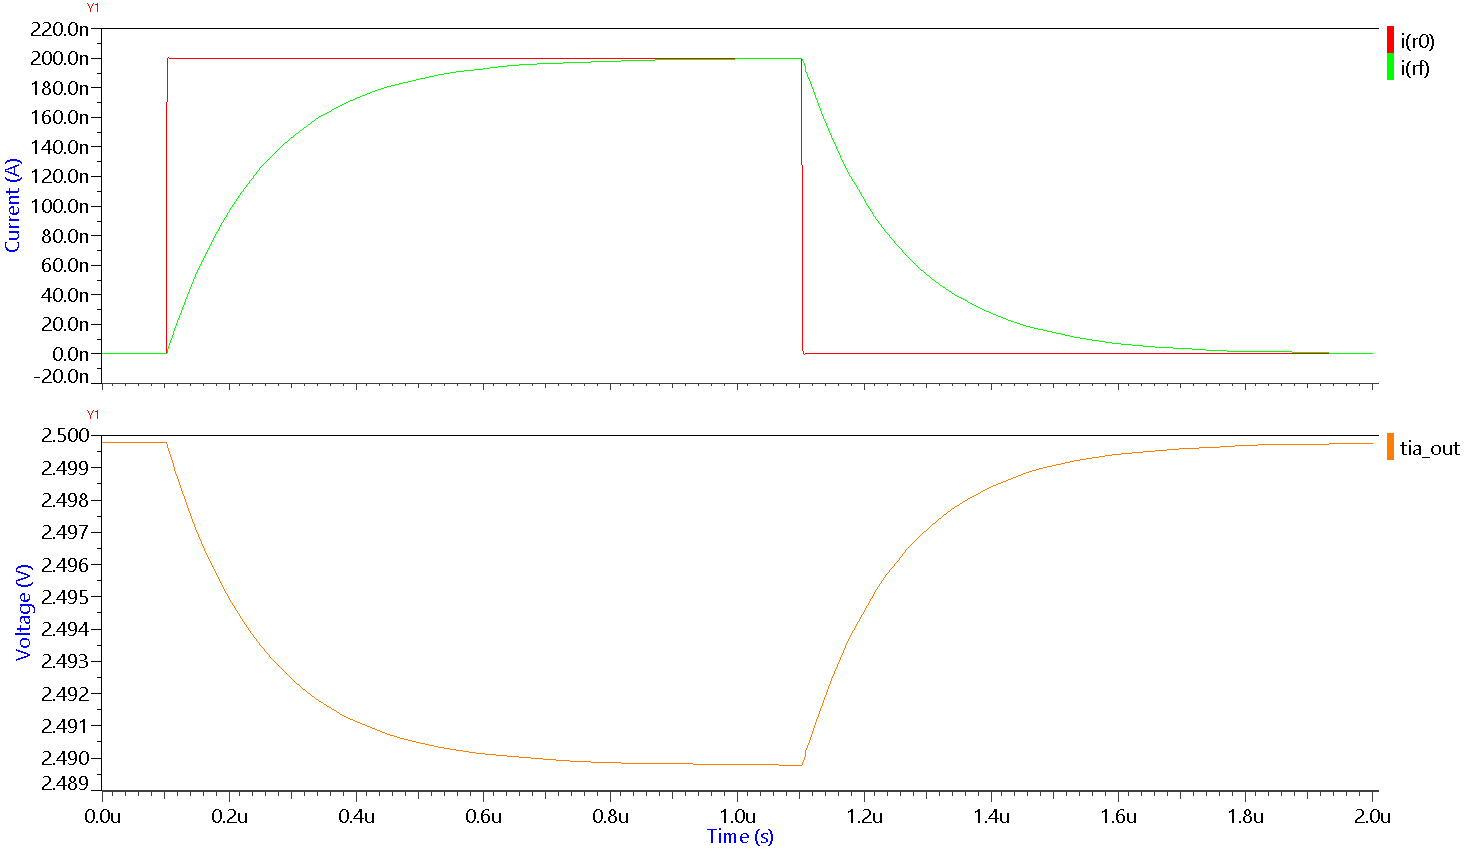
\includegraphics[width=\textwidth]{../graphics/simulation_tia_plot.png}
    \caption{Simulation \acrshort{tia} - Plot}\label{fig:simulation_tia_plot}
\end{figure}

It can be seen that the time constant of the current through the feedback resistor \lstinline|RF| according to
formula~\ref{eq:tia_tau} can be determined.

\begin{equation}\label{eq:tia_tau}
    \tau = R_F \cdot C_F = 50~k\Omega \cdot 3~pF = 150~ns
\end{equation}
\myequations{\acrshort{tia} time constant}

However, the feedback capacitor \lstinline|CF| cannot be chosen arbitrarily small, otherwise the circuit will oscillate.
Figure~\ref{fig:simulation_tia_plot_wo_cf} shows the simulation result without the feedback capacitor \lstinline|CF|.

\begin{figure}[H]
    \centering
    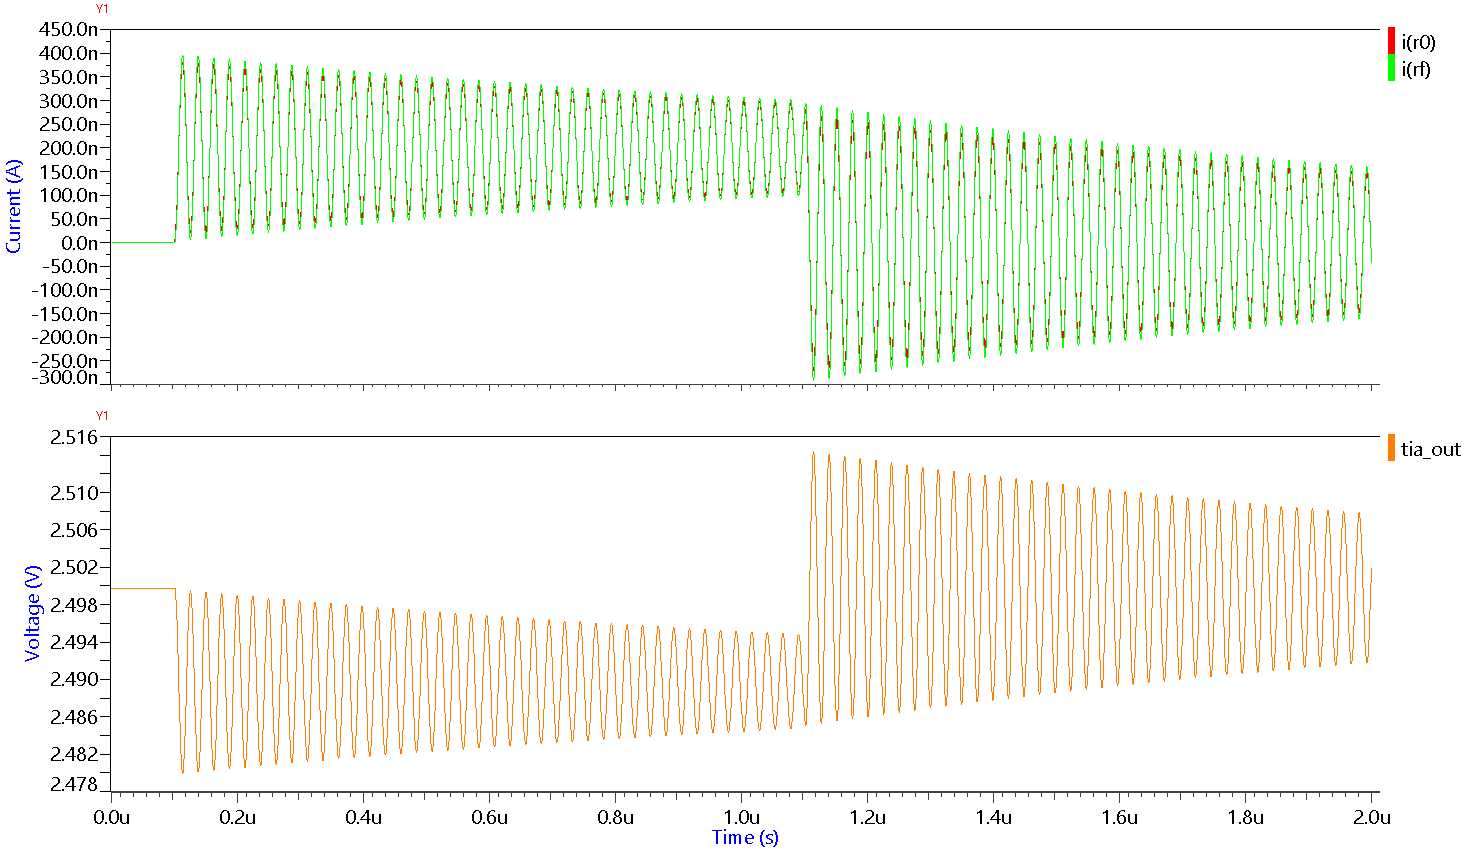
\includegraphics[width=\textwidth]{../graphics/simulation_tia_plot_wo_cf.png}
    \caption{Simulation \acrshort{tia} - Plot without \lstinline|CF|}\label{fig:simulation_tia_plot_wo_cf}
\end{figure}

The exact dimensioning of \lstinline|CF| will be determined by tests with the \acrshort{pcb}. Possibly, depending
on parasitic capacities on the \acrshort{pcb}, \lstinline|CF| will not even have to be populated.
